

%\documentclass[12pt]{article}
\documentclass[12pt]{scrartcl}
\title{ELEC 340 Assignment 3}
\nonstopmode
%\usepackage[utf-8]{inputenc}
\usepackage{graphicx} % Required for including pictures
\usepackage[figurename=Figure]{caption}
\usepackage{float}    % For tables and other floats
\usepackage{verbatim} % For comments and other
\usepackage{amsmath}  % For math
\usepackage{amssymb}  % For more math
\usepackage{fullpage} % Set margins and place page numbers at bottom center
\usepackage{paralist} % paragraph spacing
\usepackage{listings} % For source code
\usepackage{subfig}   % For subfigures
%\usepackage{physics}  % for simplified dv, and 
\usepackage{enumitem} % useful for itemization
\usepackage{siunitx}  % standardization of si units

\usepackage{tikz,bm} % Useful for drawing plots
%\usepackage{tikz-3dplot}
\usepackage{circuitikz}
\usepackage{ctable}
%%% Colours used in field vectors and propagation direction
\definecolor{mycolor}{rgb}{1,0.2,0.3}
\definecolor{brightgreen}{rgb}{0.4, 1.0, 0.0}
\definecolor{britishracinggreen}{rgb}{0.0, 0.26, 0.15}
\definecolor{cadmiumgreen}{rgb}{0.0, 0.42, 0.24}
\definecolor{ceruleanblue}{rgb}{0.16, 0.32, 0.75}
\definecolor{darkelectricblue}{rgb}{0.33, 0.41, 0.47}
\definecolor{darkpowderblue}{rgb}{0.0, 0.2, 0.6}
\definecolor{darktangerine}{rgb}{1.0, 0.66, 0.07}
\definecolor{emerald}{rgb}{0.31, 0.78, 0.47}
\definecolor{palatinatepurple}{rgb}{0.41, 0.16, 0.38}
\definecolor{pastelviolet}{rgb}{0.8, 0.6, 0.79}
\begin{document}

\begin{center}
\specialrule{0.02em}{}{}
\hrule
\vspace{0.3cm}
	{\textbf { \large {Discrete Structures (MA5.101) }}} 
\end{center}
\textbf{Instructor:}\ Dr. Ashok Kumar Das \hspace{\fill}\textbf{Assignment 1 Solutions}    \\
{\textbf{IIIT Hyderabad}   } \hspace{\fill} \textbf{Total Marks}: 50 \\ 
% keep it at the left side
\specialrule{0.01em}{}{}
\hrule

\paragraph*{Problem 1}
\small{We first define 
\begin{align*}
    & (A \Delta B)' &
    \\ &= ((A \cup B) \cap (A' \cup B'))' & \ldots \text{\{by definition\}}
    \\ &= ((A \cup B)' \cup (A' \cup B')') & \ldots \text{\{by De-Morgan's Laws\}}
    \\ &= ((A' \cap B') \cup (A \cap B)) & \ldots \text{\{by De-Morgan's Laws\}}
\end{align*}
We simplify LHS first -
\begin{align*}
    & (A \Delta B) {\Delta} C  & 
    \\ &= [(A {\Delta} B) \cap C)] \cup [(A {\Delta} B)' \cap C] & \ldots \text{\{by definition.\}}
    \\ &= [((A \cap B') \cup (A' \cap B)) {\cap} C] \cup [((A' \cap B') \cup (A \cap B)) {\cap} C] & \ldots \text{\{by definition.\}}
    \\ &= [(A \cap B' \cap C') \cup (A' \cap B \cap C')] \cup [(A' \cap B' \cap C) \cup (A \cap B \cap C)] & \ldots \text{\{distributive property\}}
    \\ &= (A \cap B' \cap C') \cup (A' \cap B \cap C') \cup(A' \cap B' \cap C) \cup (A \cap B \cap C)  & \ldots \text{\{associative property\}}
\end{align*}
We simplify RHS next - 
\begin{align*}
    & A {\Delta} (B {\Delta} C)  & 
    \\ &= [A \cap (B \Delta C)'] \cup [A' \cap (B \Delta C)] & \ldots \text{\{by definition\}}
    \\ &= [A \cap ((B' \cap C') \cup (B \cap C))] \cup [A' \cap ((A' \cap B) \cup (A \cap B'))] & \ldots \text{\{by definition\}}
    \\ &= [ ((A \cap (B' \cap C')) \cup (A \cap (B \cap C))] \cup [(A' \cap (B' \cap C)) \cup (A' \cap (B \cap C'))] & \ldots \text{\{by distributive property\}}
    \\ &= [ ((A \cap B' \cap C') \cup (A \cap B \cap C)] \cup [(A' \cap B' \cap C) \cup (A' \cap B \cap C')] & \ldots \text{\{by associative property\}}
    \\ &= (A \cap B' \cap C') \cup (A' \cap B \cap C') \cup(A' \cap B' \cap C) \cup (A \cap B \cap C) & \ldots \text{\{by commutative property\}}
\end{align*}
Hence proved.
}

\paragraph*{Problem 2}
Given:
\begin{align*} 
     A &= \{n | n \text{ is a multiple of }12\} \\ 
     B &= \{n | n\text{ is a multiple of }18\}
\end{align*}
\begin{enumerate}
    \item $A \cup B = \{n | n\text{ is a multiple of }12 \text{ or }18\}$
    \item $A \cap B = \{n | n\text{ is a multiple of }12 \text{ and }18\} = \{n | n \text{ is a multiple of }36\}$
    \item $(A - B) \cup (B - A) = A \Delta B$ \hfill \ldots\{Using Property\} \\
    $A \Delta B = \{n | n\text{ is a multiple of }12 \text{ or $n$ is a multiple of }18 \text{ but not both}\}$
    \item $A \times B = \{(a, b) | a \text{ is a multiple of }12 \text{ and $b$ is a multiple of }18\}$
    \item Multiple answers accepted here | either listing out the answer in roster form, or providing a proper set builder definition. \\ 
    \begin{align*}
        P(A \cup B) &= \Big\{ \phi &\ldots \text{(Null/Empty Set)} \\
                    & \{12\}, \{18\}, \{24\}, \{36\}, & \ldots \text{(Taken one at a time)} \\
                    & \{12, 24\}, \{18, 36\}, \{12, 18\}, & \ldots \text{(Taken two at a time)} \\
                    & \{12, 18, 24 \}, \{12, 18, 36\}, &\ldots \text{(Taken three at a time)} \\
                    & \vdots & \\
                    & \Big\}
    \end{align*}    
\end{enumerate}

\paragraph*{Problem 3}
The Venn Diagram for the problem is:
\begin{itemize}
    \item $U$ = Set of all quadrilaterals
    \item $T$ = Set of rectangles
    \item $R$ = Set of rhombuses
    \item $S$ = Set of squares
\end{itemize}
\begin{figure}[h!]
    \centering
    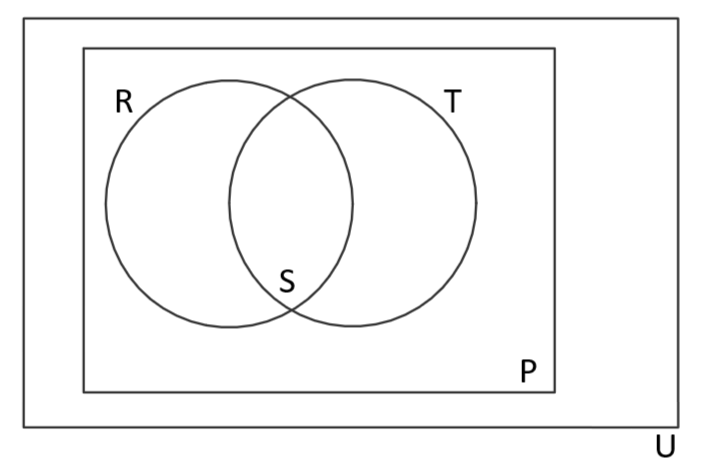
\includegraphics{venn_assgn1.png}
    \caption[width=\linewidth]{Venn Diagram of the problem}
    \label{fig:my_label}
\end{figure}
\vspace{2mm}
$P$ is defined as a quadrilateral having opposite sides parallel to each other\\
$T$ is defined as a quadrilateral having opposite sides parallel and each interior angle = $90^\circ$ \\ 
$R$ is defined as a quadrilateral having opposite sides parallel to each other and all sides equal\\
$S$ is defined as a quadrilateral having opposite sides parallel, each sides equal and each interior angle = $90^\circ$ \\

The required relations are:
\begin{enumerate}
    \item $P \subseteq U, T \subseteq U, R \subseteq U, S \subseteq U$ 
    \item $T \subseteq P, R \subseteq P$
    \item $S = R \cap T \implies (S \subseteq R) \wedge (S \subseteq T)$
\end{enumerate}

\paragraph*{Problem 4} 
Let
\begin{align*}
   E &= \text{ Set of all people who speak English }  \\
   F &= \text{ Set of all people who speak French } \\ 
   G &= \text{ Set of all people who speak German } \\
   U &= \text{ Set of all people who attended the conference }
\end{align*}
Given:
\begin{gather*}
    |E| = 28, |F| = 30, |G| = 42, |U| = 100 \\  
    |E \cap F| = 8, |F \cap G| = 5, |E \cap G| = 10 \\
    |E \cap F \cap G| = 3
\end{gather*}

\begin{enumerate}
    \item We have to calculate $|\overline{E \cup F \cup G}|$ which is given by:
    \[
        |\overline{E \cup F \cup G}| = |U| - |E \cup F \cup G|
    \]
    Now using PIE (Principle of Inclusion-Exclusion) we get:
    \begin{align*}
        |E \cup F \cup G| &= |E| + |F| + |G| - |E \cap F| - |E \cap G| - |F \cap G| + |E \cap F \cap G| \\
                          &= 28 + 30 + 42 - 8 - 5 - 10 + 3 \\
                          &= 80
    \end{align*}
    Thus the answer is:
    \begin{align*}
        |\overline{E \cup F \cup G}| &= |U| - |E \cup F \cup G| \\
                                     &= 100 - 80 \\
                                     &= 20
    \end{align*}
    \item We have to find the number of people who only speak German. The answer here is given by: 
    \begin{align*}
        \text{Ans} &= |G| - |E \cap G| - |F \cap G| + |E \cap F \cap G| \\
                   &= 42 - 10 - 5 + 3 \\ 
                   &= 30
    \end{align*}    
\end{enumerate}

\paragraph*{Problem 5}
\begin{enumerate}
    \item We first prove that $(A - B) \times C \subseteq (A \times C) - (B \times C)$
    \begin{align*}
        & (x,y) \in (A - B) \times C & 
        \\ & \implies (x \in (A - B)) \land (y \in C) & \ldots \text{\{by definition\}}
        \\ & \implies ((x \in A) \land (x \notin B)) \land (y \in C) & \ldots \text{\{by defintion of A - B\}}.
        \\ & \implies ((x \in A ) \land (y \in C)) \land  ((x \notin B)) \land (y \in C)) & \ldots \text{\{by distributivity of $\land$\}}
        \\ & \implies ((x,y) \in (A \times C)) \land ((x,y) \notin (B \times C))  & \ldots \text{\{by definition\}}
        \\ & \implies (x,y) \in (A \times C) - (B \times C) & \ldots \text{\{by definition\}}
    \end{align*}
    Now we prove that $(A \times C) - (B \times C) \subseteq (A - B) \times C$
    \begin{align*}
        & (x,y) \in (A \times C) - (B \times C) & 
        \\ & \implies ((x,y) \in (A \times C)) \land ((x,y) \notin (B \times C))  & \ldots \text{\{by definition\}}
        \\ & \implies ((x \in A ) \land (y \in C)) \land  ((x \notin B)) \land (y \in C)) & \ldots \text{\{by definition\}}
        \\ & \implies ((x \in A) \land (x \notin B)) \land (y \in C) & \ldots \text{\{by distributivity of $\land$\}}.
        \\ & \implies (x \in (A - B)) \land (y \in C) & \ldots \text{\{by definition\}}
        \\ & \implies (x,y) \in (A - B) \times C & \ldots \text{\{by definition\}}
    \end{align*}
    \item We first prove that $(A \Delta B) \times C \subseteq (A \times C) \Delta (B \times C)$
    \begin{align*}
        & (x,y) \in (A \Delta B) \times C & 
        \\ & \implies (x \in (A \Delta B)) \land (y \in C) & \ldots \text{\{by definition\}}
        \\ & \implies [((x \in A) \land (x \notin B)) \lor ((x \notin A) \land (x \in B))] \land (y \in C) & \ldots \text{\{by definition of $A  \Delta B$\}}.
        \\ & \implies [((x \in A) \land (x \notin B) \land (y \in C)) \lor ((x \notin A) \land (x \in B) \land (y \in C))] & \ldots \text{\{by distributivity of $\lor$\}}.
        \\ & \implies [(((x \in A) \land (y \in C)) \land ((x \notin B) \land (y \in C))) &
        \\ & \hspace{1.5cm} \lor (((x \notin A) \land (y \in C)) \land ((x \in B) \land (y \in C)))] & \ldots \text{\{by distributivity of $\lor$\}}.
        \\ &\implies [((x,y) \in (A \times C) - (B \times C))
        \\ & \hspace{1.5cm} \lor ((x,y) \in (B \times C) - (A \times C))] & \ldots \text{\{by definition\}}
        \\ & \implies (x,y) \in [(A \times C) - (B \times C)) \cup (B \times C) - (A \times C))] & \ldots \text{\{by definition\}}        
        \\ & \implies (x,y) \in (A \times C) \Delta (B \times C) &  \ldots \text{\{by definition\}}
    \end{align*}
    Now we prove that $(A \times C) \Delta (B \times C) \subseteq (A \Delta B) \times C$
    \begin{align*}
        & (x,y) \in (A \times C) \Delta (B \times C) & 
        \\ & \implies (x,y) \in [(A \times C) - (B \times C)) \cup (B \times C) - (A \times C))] & \ldots \text{\{by definition\}}        
        \\ &\implies [((x,y) \in (A \times C) - (B \times C))
        \\ & \hspace{1.5cm} \lor ((x,y) \in (B \times C) - (A \times C))] & \ldots \text{\{by definition\}}
        \\ & \implies [(((x \in A) \land (y \in C)) \land ((x \notin B) \land (y \in C))) &
        \\ & \hspace{1.5cm} \lor (((x \notin A) \land (y \in C)) \land ((x \in B) \land (y \in C)))] & \ldots \text{\{by definition\}}.   
        \\ & \implies [((x \in A) \land (x \notin B)) \land (y \in C)) \lor (((x \notin A) \land (x \in B)) \land (y \in C))] & \ldots \text{\{by distributivity of $\lor$\}}.
        \\ & \implies [((x \in A) \land (x \notin B)) \lor ((x \notin A) \land (x \in B))] \land (y \in C) & \ldots \text{\{by distributivity of $\lor$\}}.    
        \\ & \implies [((x \in (A - B) ) \lor ((x \in (B- A)))] \land (y \in C) & \ldots \text{\{by definition\}}
        \\ & \implies [(x \in (A - B) \cup (B - A)] \land (y \in C) & \ldots \text{\{by definition\}}
        \\ & \implies (x \in (A \Delta B)) \land (y \in C) & \ldots \text{\{by definition of $A  \Delta B$\}}
        \\ & \implies (x,y) \in (A \Delta B) \times C & \text{\{by definition\}}
    \end{align*}
\end{enumerate}

\end{document}

